\documentclass[10pt,letterpaper,twocolumn]{article}
% Standalone ML-style technical report, not an official conference submission style.
\usepackage[left=0.75in,right=0.75in,top=0.78in,bottom=0.82in,columnsep=0.25in]{geometry}
\usepackage[T1]{fontenc}
\usepackage[utf8]{inputenc}
\usepackage{amsmath,amssymb,amsthm,mathtools}
\usepackage{newtxtext,newtxmath}
\usepackage{microtype}
\usepackage{graphicx,booktabs,tabularx,array}
\usepackage{caption}
\usepackage{subcaption} 
\usepackage{enumitem,titlesec}
\usepackage{tikz}
\usetikzlibrary{arrows.meta,positioning,calc,fit,backgrounds}
\usepackage{placeins,needspace}
\usepackage[round,authoryear]{natbib}
\usepackage{xurl}
\usepackage[hidelinks]{hyperref}
\hypersetup{
  pdftitle={SETNODE: Spatial Equivariant Transformer Neural ODE for Physical Dynamics},
  pdfauthor={Trillyon Earl},
  pdfsubject={Unpublished NSF REU technical report: particle dynamics and archived-result analysis}
}
\graphicspath{{figures/}}
\setlength{\parindent}{1em}
\setlength{\parskip}{2pt}
\setlength{\textfloatsep}{11pt plus 2pt minus 2pt}
\setlength{\dbltextfloatsep}{12pt plus 2pt minus 2pt}
\setlength{\floatsep}{9pt plus 2pt minus 2pt}
\setlength{\intextsep}{10pt plus 2pt minus 2pt}
\captionsetup{font=small,labelfont=bf,skip=5pt}
\titlespacing*{\section}{0pt}{11pt plus 2pt minus 2pt}{4pt}
\titlespacing*{\subsection}{0pt}{8pt plus 2pt minus 2pt}{3pt}
\titleformat{\section}{\large\bfseries}{\thesection.}{0.5em}{}
\titleformat{\subsection}{\normalsize\bfseries}{\thesubsection.}{0.5em}{}
\setlist{nosep,leftmargin=1.4em}
\setlength{\bibsep}{4pt}
\renewcommand{\bibfont}{\small}
\pagestyle{plain}
\raggedbottom
\newtheorem{proposition}{Proposition}[section]
\newcommand{\R}{\mathbb R}
\newcommand{\LN}{\operatorname{LN}}
\newcommand{\FFN}{\operatorname{FFN}}
\newcommand{\MSE}{\operatorname{MSE}}
\newcommand{\softmax}{\operatorname{softmax}}
\newcommand{\cat}{\mathbin{\Vert}}
\newcommand{\cN}{\mathcal N}
\newcommand{\Fhat}{\widehat F}
\newcommand{\Uhat}{\widehat U}
\newcommand{\ahat}{\widehat a}
\newcommand{\norm}[1]{\lVert #1\rVert}
\numberwithin{equation}{section}
\newcolumntype{L}[1]{>{\raggedright\arraybackslash}p{#1}}
\newcolumntype{C}[1]{>{\centering\arraybackslash}p{#1}}
\emergencystretch=1.25em
\hyphenation{SETNODE EGNN}

\begin{document}
\twocolumn[{
\begin{center}
{\LARGE\bfseries SETNODE: Spatial Equivariant Transformer\\[3pt]
Neural ODE for Physical Dynamics}\\[9pt]
{\large Trillyon Earl}\\[3pt]
Saint Louis University\\[4pt]
{\small Research mentors: Dr. Qingguang Guan and Dr. Zhifu Xie\\
The University of Southern Mississippi}\\[5pt]
{\small Unpublished NSF REU technical report\enspace\textbar\enspace Summer 2026\\
Revised October 3, 2026}\\[5pt]
{\small \textbf{Code repository:}
\url{https://github.com/Branshi/REU-PhysicalAI}}
\end{center}
\vspace{8pt}
}]

\begin{abstract}
We investigate SETNODE, a Spatial Equivariant Transformer Neural ODE for learning particle dynamics.
Our graph processor combines an unnormalized sum of interaction messages with locally centered
residual attention. An invariant scalar potential yields equivariant conservative forces, and
velocity Verlet integration generates trajectories. We evaluate a force-supervised SETNODE model
and five similarly sized baselines using 3,000 two-dimensional three-body trajectories and a
reported four-hour training budget per model. The evaluated SETNODE model has 114,514 parameters,
one interaction block, two attention heads, and latent width 64. On the same 50 held-out
trajectories and 299 rollout transitions, its mean position MSE is $8.92\times10^{-5}$, 33.5\%
below our EGNN baseline, with no failures under the specified error threshold. Its mean final
center-of-mass drift is $6.61\times10^{-7}$, close to the numerical reference, although true
gravitational energy drift remains substantially larger. The findings concern the complete
model-and-solver pipelines; they do not isolate attention's contribution or establish robustness
across training seeds.
\end{abstract}

\section{Introduction}
\label{sec:intro}

\begin{figure*}[t]
\centering
\resizebox{\textwidth}{!}{% Editable SETNODE schematic. One displayed interaction block represents each of K blocks.
% N denotes particles in the paper; K denotes processor depth.
\begin{tikzpicture}[
  x=1cm,y=1cm,
  font=\sffamily\fontsize{8.2}{9.5}\selectfont,
  box/.style={draw=black!75,rounded corners=1.3pt,fill=white,
              line width=.55pt,align=center,inner sep=4pt,minimum height=.82cm},
  stage/.style={font=\sffamily\bfseries\fontsize{8}{9}\selectfont,align=center},
  substage/.style={font=\sffamily\fontsize{7.1}{8.1}\selectfont,align=center},
  arr/.style={-{Latex[length=1.7mm,width=1.2mm]},line width=.65pt},
  aux/.style={-{Latex[length=1.7mm,width=1.2mm]},line width=.55pt,draw=black!65},
  every path/.style={line cap=round,line join=round}
]
% Widen this first gap so the input label fits between, not over, the two boxes.
\node[box,text width=1.35cm] (state) at (.70,0) {Current state\\$(q_t,v_t,m)$};
\node[box,text width=1.65cm] (encoder) at (3.25,0)
  {Construct graph\\and encode\\mass features};
\node[stage] at (3.25,1.28) {ENCODER};

\node[box,text width=3.35cm,minimum height=.53cm] (edges) at (6.65,1.10)
  {Invariant edge update};
\node[box,text width=1.28cm,minimum height=.83cm] (sum) at (5.67,0)
  {Additive\\sum};
\node[box,text width=1.63cm,minimum height=.83cm] (attn) at (7.46,0)
  {Centered\\attention};
\node[box,text width=3.35cm,minimum height=.58cm] (merge) at (6.65,-1.25)
  {Residual node update\\+ feed-forward layer};
\begin{scope}[on background layer]
  \node[draw=black!45,rounded corners=2pt,fill=black!4,
        fit=(edges)(sum)(attn)(merge),inner xsep=6pt,inner ysep=5pt] (processor) {};
\end{scope}
\node[stage] at (6.65,2.10) {INTERACTION BLOCK $\times K$};
\node[substage] at (6.65,1.73) {$K=1$ in the reported experiments};

\node[box,text width=1.50cm] (potential) at (10.10,0)
  {Invariant scalar\\potential\\$\widehat U_\theta(q,m)$};
\node[stage] at (10.10,1.28) {READOUT};
\node[box,text width=1.62cm] (force) at (12.30,0)
  {Coordinate gradient\\then force / mass};
\node[stage] at (12.30,1.28) {DYNAMICS};
\node[box,text width=1.48cm] (solver) at (14.60,0)
  {Velocity Verlet\\integration};
\node[stage] at (14.60,1.28) {SOLVER};
\node[box,text width=1.47cm] (next) at (16.85,0)
  {Next state\\$(q_{t+\Delta t},$\\$v_{t+\Delta t},m)$};

\draw[arr] (state.east) -- node[midway,above=3pt,inner sep=1pt,
  font=\fontsize{7.3}{8.2}\selectfont] {$q_t,m$} (encoder.west);
\draw[arr] (encoder.east) -- (4.49,0) |- (edges.west);
\draw[arr] (edges.south) -- (6.65,.635) -| (sum.north);
\draw[arr] (6.65,.635) -| (attn.north);
\draw[arr] (sum.south) -- (5.67,-.63) -| (merge.north);
\draw[arr] (attn.south) -- (7.46,-.63) -| (merge.north);
\draw[arr] (merge.east) -- (8.82,-1.25) |- (potential.west);
\draw[arr] (potential.east) -- (force.west);
\draw[arr] (force.east) -- (solver.west);
\draw[arr] (solver.east) -- (next.west);

% Velocities enter the solver, not the potential network.
\draw[aux] (state.north) -- (.70,2.62) -- (15.53,2.62) -- (15.53,.82)
  -- (14.60,.82) -- (solver.north);
\node[fill=white,inner sep=2pt,font=\fontsize{8}{9}\selectfont] at (10.78,2.62)
  {$q_t,v_t$ to the integrator};

% Rollout feedback is separate from stacking K interaction blocks.
\draw[aux,dashed] (next.south) -- (16.85,-2.08) -- (.70,-2.08) -- (state.south);
\node[fill=white,inner sep=2.5pt,font=\fontsize{8}{9}\selectfont] at (9.55,-2.08)
  {Repeat the state update to generate a trajectory};
\end{tikzpicture}
}
\caption{\textbf{SETNODE architecture.} We encode the particle graph, update its latent features
through unnormalized-sum and centered-attention branches, and read out an invariant scalar potential.
Differentiating the potential gives forces, which are divided by particle masses to obtain
accelerations. Velocity Verlet uses this learned acceleration field and the current state to advance
the system, reevaluating the force within each step. The processor supports $K$ blocks;
our evaluated model uses $K=1$. Velocities enter the integrator, not the potential network.
Repeating the state update generates a trajectory.}
\label{fig:architecture}
\end{figure*}

Learning physical dynamics requires a model to represent interactions among objects and remain
accurate when its predictions are repeatedly integrated over time. Graph networks represent
particles as nodes and interactions as edges \citep{battaglia2018relational,sanchezgonzalez2020learning}.
Equivariant graph networks constrain predictions to transform consistently with the coordinate
system \citep{satorras2021en}. Neural ODEs represent continuous-time dynamics with a learned vector
field and use a numerical solver to generate trajectories \citep{chen2018neural}. Energy-based
models add structure by obtaining dynamics from derivatives of a learned scalar function
\citep{greydanus2019hamiltonian}.

We combine these ideas with attention \citep{vaswani2017attention,velickovic2018graph} in SETNODE
(Figure~\ref{fig:architecture}). Our design has two complementary goals: to accumulate interaction
information in a way motivated by physics, and to adjust that representation to the current
configuration. The first goal follows from force additivity. Net force is a sum of contributions,
not an average whose weights must sum to one. We therefore keep an explicit unnormalized sum of
learned interaction messages. This does not mean normalized attention cannot learn forces; our
hypothesis is that an additive pathway makes their structure more natural to represent.

For the second goal, we apply the subtract-uniform centering operation studied by
\citet{ali2023centered} to local interaction messages. Each head subtracts the uniform neighbor
weight from its softmax weights, so its output is an attention-weighted average minus a uniform
average. This lets the model represent departures from treating all neighbors equally, while keeping
a separate additive pathway. We intend attention to provide context-sensitive adjustments when
particular interactions matter for predicting the dynamics, including uncommon configurations.
Centering itself does not measure rarity, and the two branches are not forced to specialize in
ordinary and unusual interactions.

A fluid confined in a box motivates future experiments. Suppose fluid--fluid interactions dominate
the training samples, while fluid--wall interactions are less common. With suitable boundary
features, attention could help represent these less prevalent but consequential interactions while
the additive branch continues to aggregate all messages. This is a hypothesis for future
fluid--boundary experiments, not a capability established by our three-body study. Such an extension
also requires suitable modeling of boundary conditions and nonconservative dynamics.

Both branches act on latent features rather than independently identified physical forces. Their
outputs contribute to an invariant potential, whose negative coordinate gradient supplies the
learned force field. We use the three-body problem as a controlled setting for studying these
representation and aggregation choices, not as a claim that a learned model should replace a
numerical solver when the exact force law is already known.

\paragraph{Related work and scope.}
\citet{ali2023centered} introduced subtract-uniform attention to address oversmoothing, in which
repeated aggregation makes representations increasingly similar. Our centered heads use that same
centering operation locally. Differential Transformer
\citep{ye2025differential} also forms a difference of attention maps, but subtracts a second learned
softmax map rather than a uniform baseline.

Equivariant attention and continuous-time dynamics also have direct precedents. TorchMD-NET
\citep{tholke2022equivariant} uses an equivariant transformer for molecular potentials and replaces
softmax with SiLU in its attention weights. Thus attention need not use normalized weights.
SEGNO \citep{liu2024segno} combines equivariant graph networks with second-order continuous-time
dynamics. Our focus is the implemented combination of an explicit additive branch, locally
centered attention, and an invariant-potential readout, together with a documented preliminary
evaluation of rollout accuracy and conservation. Controlled ablations and repeated training are
future tasks needed to identify which components provide reliable benefits.

\Needspace{11\baselineskip}
\section{Notation and Framework}
\label{sec:framework}

We consider $N$ particles with positions $q_i\in\R^d$, velocities $v_i\in\R^d$, and constant positive
masses $m_i$. Our dataset uses $N=3$, $d=2$, and gravitational constant $G=1$, without physical
softening. Away from collisions, the dynamics and potential are
\begin{equation}
\begin{aligned}
\dot q_i &= v_i,\\
\dot v_i &= G\sum_{j\ne i}m_j\frac{q_j-q_i}{\norm{q_j-q_i}^{3}},\\
U(q,m) &= -G\sum_{i<j}\frac{m_im_j}{\norm{q_j-q_i}}.
\end{aligned}
\label{eq:physical}
\end{equation}
The physical force is $F_i=-\nabla_{q_i}U=m_i\dot v_i$.

Our graph contains every directed edge $j\to i$ with $j\ne i$. Thus
$\cN(i)=\{j:j\ne i\}$ and $|\mathcal E|=N(N-1)$. We use raw masses as node features,
$x_i=[m_i]$, and sender--receiver masses as edge features, $a_{ij}=[m_j,m_i]$.
We standardize these features using means and standard deviations computed only from the training
set. Learned MLP encoders then map them to 64-dimensional node and edge representations.

Geometry enters through pairwise radial quantities,
\begin{equation}
d_{ij}^2=\norm{q_j-q_i}^2,\qquad
r_{ij}^{-1}=\frac{1}{\norm{q_j-q_i}},
\label{eq:radial}
\end{equation}
rather than raw coordinates passed to a generic MLP. In the implementation, the squared distance is
clamped from below at $10^{-12}$ when computing the inverse distance. This numerical safeguard
avoids division by zero and sufficiently small distances.

We write $Q\in O(d)$ for an orthogonal matrix, satisfying $Q^\top Q=I$, and $b\in\R^d$ for a
translation. A Euclidean coordinate change applies $q_i\mapsto Qq_i+b$ to every particle. The
scalar potential should remain unchanged, while the forces should rotate or reflect with $Q$.
Similarly, a particle permutation must leave the potential unchanged and permute the associated
forces. We learn a position- and mass-dependent potential. The kinetic-energy term is known,
and velocities enter the integrator rather than the potential network.

\section{SETNODE Method}
\label{sec:method}

\subsection{Invariant edge updates and dual aggregation}

Let $h_i$ and $e_{ij}$ be the latent node and edge vectors, and let $\bar h_i=\LN(h_i)$, where
$\LN$ denotes layer normalization. A shared MLP updates each edge:
\begin{equation}
\widetilde e_{ij}=e_{ij}+\phi_e\!\left(
\bar h_i\cat\bar h_j\cat r_{ij}^{-1}\cat d_{ij}^2\cat e_{ij}\right).
\label{eq:edge}
\end{equation}
Here $\cat$ denotes concatenation. The additive branch then computes
\begin{equation}
\begin{aligned}
M_{i,\Sigma}&=\sum_{j\in\cN(i)}\widetilde e_{ij},\\
\Delta_{i,\Sigma}&=\phi_\Sigma(\bar h_i\cat M_{i,\Sigma}).
\end{aligned}
\label{eq:sum}
\end{equation}
This preserves an unnormalized sum of interaction messages. The nonlinear MLP does
not require the branch's output to be a sum of independent force contributions.

For attention head $a\in\{1,\ldots,H\}$, we compute
\begin{equation}
\begin{aligned}
z_{ij}^a&=W^a[\bar h_i\cat\bar h_j\cat\widetilde e_{ij}]+b^a,\\
s_{ij}^a&=(w^a)^\top\operatorname{LeakyReLU}_{0.2}(z_{ij}^a),\\
\alpha_{ij}^a&=\softmax_{j\in\cN(i)}(s_{ij}^a).
\end{aligned}
\label{eq:score}
\end{equation}
The centered head output is
\begin{equation}
C_i^a=\sum_{j\in\cN(i)}\left(\alpha_{ij}^a-\frac{1}{n_i}\right)
V^a(\widetilde e_{ij}),\qquad n_i=|\cN(i)|.
\label{eq:center}
\end{equation}
Here $V^a(e)=W_V^a e+b_V^a$ is a learned value projection. We concatenate the heads,
apply a learned output projection, and compute the attention-branch update:
\begin{equation}
\begin{aligned}
C_i&=W_O[C_i^1\cat\cdots\cat C_i^H]+b_O,\\
\Delta_{i,A}&=\phi_A(\bar h_i\cat C_i).
\end{aligned}
\label{eq:attnupdate}
\end{equation}
The two branches are combined in a residual update,
\begin{equation}
\begin{aligned}
u_i&=h_i+\Delta_{i,\Sigma}+\gamma\odot\Delta_{i,A},\\
h_i^+&=u_i+\FFN(\LN(u_i)),
\end{aligned}
\label{eq:node}
\end{equation}
where $\odot$ is elementwise multiplication and $\FFN$ is a feed-forward network. We initialize
every entry of the LayerScale vector $\gamma$ to $10^{-2}$ \citep{touvron2021going}. The MLPs and
feed-forward layer use SiLU activations; the attention scores use LeakyReLU.

The processor can contain $K$ interaction blocks. Equations~\eqref{eq:edge}--\eqref{eq:node}
describe one block; successive blocks update the features passed to the readout. Our evaluated
model uses $K=1$, latent and hidden widths of 64, two attention heads of width 32, and feed-forward
width 128. Its configurable MLPs have one hidden layer. Table~\ref{tab:models} and
Appendix~\ref{app:record} summarize the saved settings.

\subsection{Potential readout and physical forces}

The potential readout has a separate residual edge update. Let $h_i^{\rm final}$ and
$e_{ij}^{\rm final}$ denote the features after the last interaction block; for $K=1$, these are
$h_i^+$ and $\widetilde e_{ij}$. With $\widetilde h_i=\LN(h_i^{\rm final})$, we write
\begin{equation}
e^R_{ij}=e^{\rm final}_{ij}+\phi_R\!\left(
\widetilde h_i\cat\widetilde h_j\cat r_{ij}^{-1}\cat d_{ij}^2\cat e^{\rm final}_{ij}\right).
\label{eq:readoutedge}
\end{equation}
The scalar network output is
\begin{equation}
\begin{aligned}
V_\theta(q,m)&=\sum_i\psi_{\rm node}(\widetilde h_i)\\
&\quad+\sum_{i<j}\psi_{\rm pair}\!\left(
\frac{e^R_{ij}+e^R_{ji}}{2}\cat\rho(d_{ij}^2)\right).
\end{aligned}
\label{eq:potential}
\end{equation}
The radial embedding $\rho$ has MLP widths $1\to32\to8$. Averaging the two directed messages
makes each unordered pair contribution symmetric. Although the final readout is summed over particle pairs, each pair's latent representation can contain 
information from other particles through message passing. The learned potential can therefore represent many-body interactions rather than only independent 
pairwise terms.

The network predicts normalized force. Using the saved scalar scale
$\sigma_F\simeq1.412318$, we restore physical units:
\begin{equation}
\begin{aligned}
\Fhat_{i,\mathrm{norm}}&=-\nabla_{q_i}V_\theta,&
\Uhat_\theta&=\sigma_F V_\theta,\\
\Fhat_i&=\sigma_F\Fhat_{i,\mathrm{norm}}=-\nabla_{q_i}\Uhat_\theta,&
\ahat_i&=\Fhat_i/m_i.
\end{aligned}
\label{eq:normalization}
\end{equation}
A fixed scalar rescaling preserves the force's geometric transformation properties. During training,
we retain the computation graph of the coordinate derivative so that backpropagation can
differentiate the force loss with respect to the network parameters.

\subsection{Generating trajectories}

Starting from $(q_t,v_t)$, we use velocity Verlet to advance the state:
\begin{equation}
\begin{aligned}
a_t&=\ahat_\theta(q_t,m),\\
q_{t+\Delta t}&=q_t+\Delta t\,v_t+\tfrac12\Delta t^2a_t,\\
a_{t+\Delta t}&=\ahat_\theta(q_{t+\Delta t},m),\\
v_{t+\Delta t}&=v_t+\tfrac12\Delta t(a_t+a_{t+\Delta t}).
\end{aligned}
\label{eq:verlet}
\end{equation}
We do not use temporal attention. For the simulated system, the current positions, velocities, and
masses provide the state needed to determine its dynamics. Our network models spatial interactions
at the current configuration, and repeated numerical integration generates the trajectory.

\section{Structural Properties}
\label{sec:properties}

The following propositions verify the intended properties of our construction, rather than
introduce new general results about invariant potentials. We ignore floating-point rounding
errors. Derivative-based statements apply where the learned potential is differentiable.
Continuous-time results assume fixed model parameters and masses, along trajectories where the
required derivatives exist. We give the proofs in Appendix~\ref{app:proofs}.

\begin{samepage}
\begin{proposition}[Centered attention head]
\label{prop:centered}
For a receiver $i$ with $n_i>0$ neighbors and head $a$,
\begin{equation}
\sum_{j\in\cN(i)}\left(\alpha_{ij}^a-\frac{1}{n_i}\right)=0.
\label{eq:zerosum}
\end{equation}
Consequently,
\begin{equation}
C_i^a=\sum_j\alpha_{ij}^aV^a(\widetilde e_{ij})
-\frac{1}{n_i}\sum_jV^a(\widetilde e_{ij}).
\label{eq:diffaverages}
\end{equation}
The head output is zero when all neighbor value vectors are identical.
\end{proposition}
\end{samepage}

This property belongs to the centered head, not necessarily the full attention branch. The output
projection has a bias, and $\phi_A$ also receives $\bar h_i$. Thus $\Delta_{i,A}$ can be nonzero
even when every head is zero. By contrast, the value-projection bias $b_V^a$ cancels inside
each head because its coefficients sum to zero. This cancellation does not remove the
output-projection bias $b_O$.

\begin{samepage}
\begin{proposition}[Invariant potential]
\label{prop:potential}
For any orthogonal matrix $Q\in O(d)$ and translation $b\in\R^d$,
\begin{equation}
\Uhat_\theta(Qq+b,m)=\Uhat_\theta(q,m).
\label{eq:uinvariant}
\end{equation}
For a particle permutation $P$ applied jointly to positions and masses,
\begin{equation}
\Uhat_\theta(Pq,Pm)=\Uhat_\theta(q,m).
\label{eq:upermutation}
\end{equation}
\end{proposition}
\end{samepage}

The potential is unchanged by translating, rotating, reflecting, or consistently relabeling the
system. Forces, however, must transform with the particles.

\begin{samepage}
\begin{proposition}[Equivariant force]
\label{prop:force}
The force $\Fhat_i=-\nabla_{q_i}\Uhat_\theta$ satisfies
\begin{equation}
\begin{aligned}
\Fhat_i(Qq+b,m)&=Q\Fhat_i(q,m),\\
\Fhat_\theta(Pq,Pm)&=P\Fhat_\theta(q,m).
\end{aligned}
\label{eq:fequivariant}
\end{equation}
\end{proposition}
\end{samepage}

Thus rotating or reflecting the system rotates or reflects its predicted forces, while relabeling
particles relabels the outputs. The potential is permutation-invariant; the forces are
permutation-equivariant.

\begin{samepage}
\begin{proposition}[Momentum and center of mass]
\label{prop:momentum}
Translation invariance of $\Uhat_\theta$ implies
\begin{equation}
\sum_i\Fhat_i=0.
\label{eq:netforce}
\end{equation}
Under $\dot q_i=v_i$ and $m_i\dot v_i=\Fhat_i$, total momentum is constant and the center of mass
moves at constant velocity:
\begin{equation}
\frac{d}{dt}\sum_i m_iv_i=0,\qquad
\ddot q_{\rm cm}=0,\qquad
q_{\rm cm}=\frac{\sum_i m_iq_i}{\sum_i m_i}.
\label{eq:momentum}
\end{equation}
\end{proposition}
\end{samepage}

The center of mass remains fixed only when its initial velocity is zero.

\begin{samepage}
\begin{proposition}[Conservation of learned energy]
\label{prop:energy}
Define the learned energy by
\begin{equation}
\widehat H(q,v,m)=\sum_i\tfrac12m_i\norm{v_i}^2+\Uhat_\theta(q,m).
\label{eq:learnedenergy}
\end{equation}
Along the continuous-time dynamics $\dot q_i=v_i$ and
$m_i\dot v_i=-\nabla_{q_i}\Uhat_\theta$, we have $d\widehat H/dt=0$.
\end{proposition}
\end{samepage}

These properties do not guarantee an accurate physical force law. Conservation of the
\emph{learned} energy is distinct from conservation of the true gravitational energy. A finite-step
numerical solver need not conserve either energy exactly.

\section{Experimental Methods}
\label{sec:experiments}

\subsection{Dataset and partitioning}

Our dataset contains 3,000 two-dimensional three-body trajectories, each with 300 saved states at
intervals of $\Delta t=0.01$. A seeded trajectory-level split assigns 2,100 trajectories to training,
450 to validation, and 450 to testing. The partitions are disjoint and cover the full dataset; all
six checkpoints store the same split manifest. The accompanying generator uses velocity Verlet
and shifts initial positions and velocities to the center-of-mass frame. Table~\ref{tab:data}
lists the saved generation settings.

\begin{table}[htbp]
\centering\small
\caption{Saved three-body dataset settings, in simulation units. The generator applies the
acceleration threshold to individual coordinate components.}
\label{tab:data}
\setlength{\tabcolsep}{4pt}
\begin{tabular}{lr}
\toprule
Setting & Value\\
\midrule
Gravitational constant $G$ & 1.0\\
Physical softening $\varepsilon$ & 0.0\\
Position / velocity initialization scales & 0.8 / 0.8\\
Initial / trajectory separation thresholds & 0.4 / 0.3\\
Maximum acceleration threshold & 100.0\\
Rejected candidate trajectories & 14,276\\
Generation / split seeds & 42 / 42\\
\bottomrule
\end{tabular}
\end{table}

\subsection{Our baseline implementations}

We implemented GNS, EGNN, EGNN-HNN, HNN, and a global MLP in our project codebase. They follow
the general ideas of their model families, rather than reproducing the exact published benchmark
configurations. The code and evaluation records name our EGNN baseline \texttt{EGNS}; we use
\emph{EGNN} throughout the paper.

\textbf{GNS} predicts acceleration from node features containing velocity and mass. Its eight edge
features include relative displacement, radial quantities, sender mass, and analytic pairwise
gravitational-acceleration components. \textbf{EGNN} uses mass and invariant radial features with
geometric vector updates. \textbf{EGNN-HNN} combines graph processing with an invariant potential
and coordinate differentiation.

Our \textbf{HNN} is a dense potential model. It takes six position coordinates and three masses,
uses three width-235 Tanh hidden layers, and outputs a scalar. It does not impose Euclidean or
permutation symmetry. Our \textbf{MLP} takes positions, velocities, and masses (15 inputs), uses
three width-234 Tanh hidden layers, and predicts six acceleration coordinates.

\begin{table*}[t]
\centering\small
\caption{\textbf{Evaluated model settings.} For graph models, width is the node/edge latent dimension
and the common hidden width of the configurable MLPs. For dense models, it is the number of units
in each hidden layer. Blocks count interaction processors. Batch size is the
number of states used per optimizer update. F and A denote force and acceleration targets.
Parameter counts exclude normalization buffers.}
\label{tab:models}
\setlength{\tabcolsep}{9pt}
\begin{tabular}{lrrrrcl}
\toprule
Model & Width & Blocks & Batch size & Parameters & Target & Integrator\\
\midrule
GNS & 43 & 6 & 4 & 114,597 & A & RK4\\
EGNN & 40 & 6 & 4 & 116,006 & A & RK4\\
EGNN-HNN & 41 & 6 & 4 & 116,647 & F & Velocity Verlet\\
HNN & 235 & --- & 256 & 113,506 & F & Velocity Verlet\\
MLP & 234 & --- & 256 & 115,134 & A & RK4\\
SETNODE & 64 & 1 & 4 & 114,514 & F & Velocity Verlet\\
\bottomrule
\end{tabular}
\end{table*}

As Table~\ref{tab:models} shows, the six models have similar parameter counts but different inputs,
depths, batch sizes, objectives, and integrators. We therefore evaluate complete model-and-solver
pipelines under the same reported time budget.
In particular, GNS receives analytic pairwise gravitational-acceleration features. It is a
physics-feature-augmented baseline. These features are computed from the current state, rather than taken from future states.

\subsection{Instantaneous supervision and model selection}

We train the models to predict the instantaneous force or acceleration at sampled states. The
checkpoint filenames call this stage \texttt{one\_step}, but its loss fits neither the next state
directly nor an entire trajectory. No rollout fine-tuning is included in the reported results.

Each model has a reported four-hour training budget on a MacBook M3 Max.\footnote{The archived checkpoints do not record exact elapsed training time or completed epoch counts, so the four-hour duration is taken from the experiment record rather than independently verified.}
We use Adam with learning rate $10^{-4}$ and saved training seed 42. Each graph-model batch
averages the loss over four sampled trajectory--time states, with 1,000 updates configured per
epoch. The dense HNN and MLP trainers use batches of 256 states. We compute normalization
statistics only on the training partition and save them with the models.

SETNODE, EGNN-HNN, and HNN use normalized force MSE:
\begin{equation}
\mathcal L_F=\MSE\!\left(\Fhat_{\rm norm},\frac{ma}{\sigma_F}\right),
\quad \sigma_F\simeq1.412318.
\label{eq:force_loss}
\end{equation}
Here $ma$ is the physical force target and $\sigma_F$ is its training-set normalization scale.
GNS, EGNN, and MLP instead use normalized acceleration MSE:
\begin{equation}
\mathcal L_a=\MSE\!\left(\ahat_{\rm norm},\frac{a}{\sigma_a}\right),
\quad \sigma_a\simeq1.130909,
\label{eq:acc_loss}
\end{equation}
with zero acceleration-target mean. We also record acceleration errors in physical units for all
models. Force and acceleration supervision weight the examples differently when masses vary.
Since $\Fhat_i-F_i=m_i(\ahat_i-a_i)$, each particle's contribution to normalized force MSE is
proportional to
\begin{equation}
\frac{m_i^2}{\sigma_F^2}\norm{\ahat_i-a_i}^2.
\label{eq:massweight}
\end{equation}
Force supervision therefore emphasizes acceleration errors for higher-mass particles. Our SETNODE
checkpoint uses the force objective, not the hybrid force--acceleration objective in separate
experimental variants.

All six models use the same ordered set of 500 validation trajectory--time pairs, selected with
validation seed 1234. We keep each model's checkpoint with the lowest recorded normalized
validation objective for its target. The evaluation uses these saved one-step checkpoints.

\subsection{Rollout protocol and metrics}
\label{sec:eval}

We use the first 50 trajectories in the saved test-manifest order. Every model starts from the same
true initial position and velocity for each trajectory and predicts $T=299$ transitions, covering
2.99 simulation-time units. We exclude the initial state from prediction error. For trajectory $r$,
\begin{equation}
E_r^q=\frac{1}{TNd}\sum_{t=1}^{T}\sum_{i=1}^{N}
\norm{\widehat q_{r,t,i}-q_{r,t,i}}^2.
\label{eq:mse}
\end{equation}
We report the mean, population standard deviation, and median of $E_r^q$ across the 50 trajectories.
We count a trajectory as a failure if a predicted position, velocity, or acceleration becomes NaN
or infinite, or if the maximum position RMSE over the rollout exceeds 0.1. We measure acceleration error on all 300 saved true
states, separately from the rollout error.

Conservation diagnostics use the true gravitational energy,
\begin{equation}
H(q,v,m)=\sum_i\tfrac12m_i\norm{v_i}^2+U(q,m),
\label{eq:trueenergy}
\end{equation}
not the learned potential. We record final absolute energy drift $|H_T-H_0|$, relative energy drift
$|H_T-H_0|/\max\{|H_0|,10^{-8}\}$, and center-of-mass displacement
$\norm{q_{{\rm cm},T}-q_{{\rm cm},0}}$. The latter is interpreted for the generator's zero-momentum
initialization. Applying the same diagnostics to the saved numerical trajectories gives a reference. We compute the reported summaries from the saved per-trajectory
evaluation records.

\section{Empirical Results}
\label{sec:results}

\subsection{Prediction accuracy and failures}

SETNODE has the lowest mean and median rollout position MSE in our fixed test suite
(Table~\ref{tab:results}). Its mean error is 33.5\% below EGNN and 61.8\% below EGNN-HNN. The
advantage is not uniform: SETNODE has lower error than EGNN on 30 of 50 paired trajectories and
lower error than EGNN-HNN on 32 of 50.

\begin{table}[t]
\centering\fontsize{8.6}{10}\selectfont
\caption{Rollout position MSE on the same 50 trajectories. SD is the population standard deviation
across trajectories. Failures follow Section~\ref{sec:eval}.}
\label{tab:results}
\setlength{\tabcolsep}{3pt}
\begin{tabular}{lrrrr}
\toprule
Model & Mean & SD & Median & Failures\\
\midrule
% BEGIN RESULTS_ROWS
GNS & $1.81\times 10^{-3}$ & $1.81\times 10^{-3}$ & $1.27\times 10^{-3}$ & 14/50 \\
EGNN & $1.34\times 10^{-4}$ & $1.74\times 10^{-4}$ & $5.22\times 10^{-5}$ & 0/50 \\
EGNN-HNN & $2.33\times 10^{-4}$ & $5.57\times 10^{-4}$ & $7.50\times 10^{-5}$ & 1/50 \\
HNN & $4.71\times 10^{-4}$ & $6.34\times 10^{-4}$ & $1.90\times 10^{-4}$ & 4/50 \\
MLP & $7.61\times 10^{-4}$ & $1.09\times 10^{-3}$ & $4.26\times 10^{-4}$ & 4/50 \\
\textbf{SETNODE} & $8.92\times 10^{-5}$ & $1.14\times 10^{-4}$ & $3.19\times 10^{-5}$ & 0/50 \\
% END RESULTS_ROWS
\bottomrule
\end{tabular}
\end{table}

The error distributions overlap substantially among the equivariant models, and some trajectories
have much larger errors than the median (Figure~\ref{fig:distribution}). SETNODE and EGNN have no
failures under our threshold. None of the six models has a recorded NaN or infinite prediction in
this suite: all recorded failures exceed the position-error threshold. Zero failures on these
50 trajectories does not guarantee stability on other trajectories or longer rollouts.

\begin{figure*}[t]
\centering
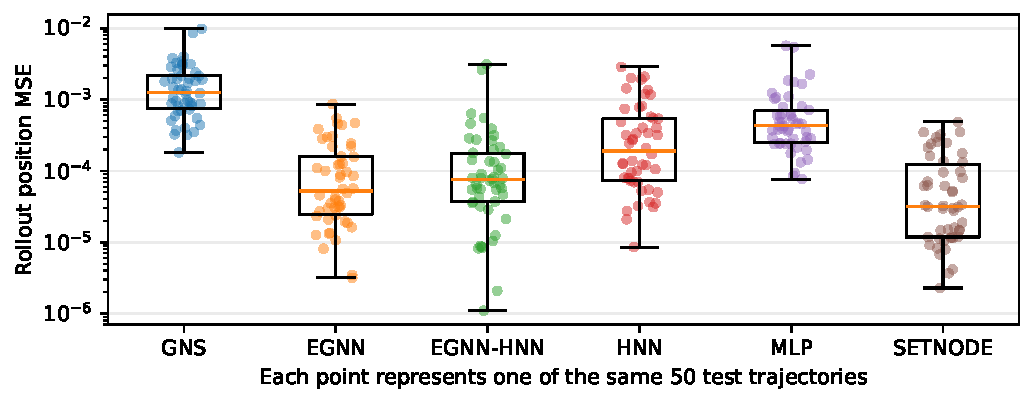
\includegraphics[width=.88\textwidth]{rollout_error_distribution.pdf}
\caption{\textbf{Distribution of rollout position errors.} Each dot represents one of the same
50 test trajectories; horizontal jitter is used only for visibility. Boxes show the interquartile
range and median, and whiskers span the observed range. The vertical axis is logarithmic. We show
one evaluated checkpoint per architecture.}
\label{fig:distribution}
\end{figure*}

\subsection{Conservation behavior}

SETNODE and EGNN-HNN have mean final center-of-mass drifts of approximately $6\times10^{-7}$,
close to the numerical reference (Table~\ref{tab:conservation}). This is consistent with the zero
total force implied by a translation-invariant potential. It does not establish accurate relative
motion: an incorrect force field can still preserve the center of mass.

\begin{table}[t]
\centering\fontsize{8.6}{10}\selectfont
\caption{Mean final conservation diagnostics. Absolute energy drift and center-of-mass drift use
simulation units; relative drift is dimensionless. The numerical reference uses the saved
true-trajectory diagnostics from SETNODE's evaluation.}
\label{tab:conservation}
\setlength{\tabcolsep}{3.2pt}
\begin{tabular}{lrrr}
\toprule
Model & Absolute & Relative & Center of mass\\
 & energy drift & energy drift & drift\\
\midrule
% BEGIN CONSERVATION_ROWS
GNS & $5.07\times 10^{-2}$ & $5.08\times 10^{-1}$ & $7.11\times 10^{-2}$ \\
EGNN & $7.71\times 10^{-3}$ & $6.36\times 10^{-2}$ & $7.82\times 10^{-3}$ \\
EGNN-HNN & $1.32\times 10^{-2}$ & $1.85\times 10^{-1}$ & $6.04\times 10^{-7}$ \\
HNN & $1.49\times 10^{-2}$ & $1.33\times 10^{-1}$ & $5.24\times 10^{-3}$ \\
MLP & $4.03\times 10^{-2}$ & $5.90\times 10^{-1}$ & $2.04\times 10^{-2}$ \\
SETNODE & $7.35\times 10^{-3}$ & $1.51\times 10^{-1}$ & $6.61\times 10^{-7}$ \\
\midrule
Numerical reference & $7.58\times 10^{-5}$ & $1.01\times 10^{-3}$ & $6.19\times 10^{-7}$ \\
% END CONSERVATION_ROWS
\bottomrule
\end{tabular}
\end{table}

SETNODE's mean absolute energy drift is $7.35\times10^{-3}$, slightly below EGNN's but about
97 times the numerical reference. The ordering changes for mean \emph{relative} energy drift:
EGNN obtains 0.0636 and SETNODE obtains 0.151. SETNODE's median relative drift is 0.00487, much
smaller than its mean; its largest value is 5.94 on trajectory 2085. Relative normalization can
emphasize trajectories with small initial energy, so absolute and relative drift answer different
questions.

Imperfect force fitting and finite-step integration can both contribute to energy drift. Our
experiment does not separate their effects. In particular, conservation of the learned energy in
continuous time does not imply conservation of the true gravitational energy measured here.

\subsection{Illustrative rollouts with an extended potential readout}
\label{sec:later_rollouts}

Figure~\ref{fig:later_rollouts} shows two illustrative trajectories from
later SETNODE variants trained for approximately 12 hours on a M3 Macbook Max. These variants
use an extended potential readout with four changes. First, we apply the
shared pair-scoring MLP to the two directed pair representations separately,
then average the resulting scalar scores, rather than averaging the
representations before scoring. Second, we use a multiscale distance
embedding. Third, skip connections give the readout direct access to the
original normalized node and edge features alongside the processed latents.
Finally, learned gates combine node, pair, and global energy contributions,
with the global term computed from pooled latent features.

These examples are separate from the four-hour evaluation and are not
included in its summary statistics. Because both the training duration and
readout differ, these images do not isolate the effects of either change.

\begin{figure*}[t]
    \centering
    \begin{subfigure}[t]{0.49\textwidth}
        \centering
        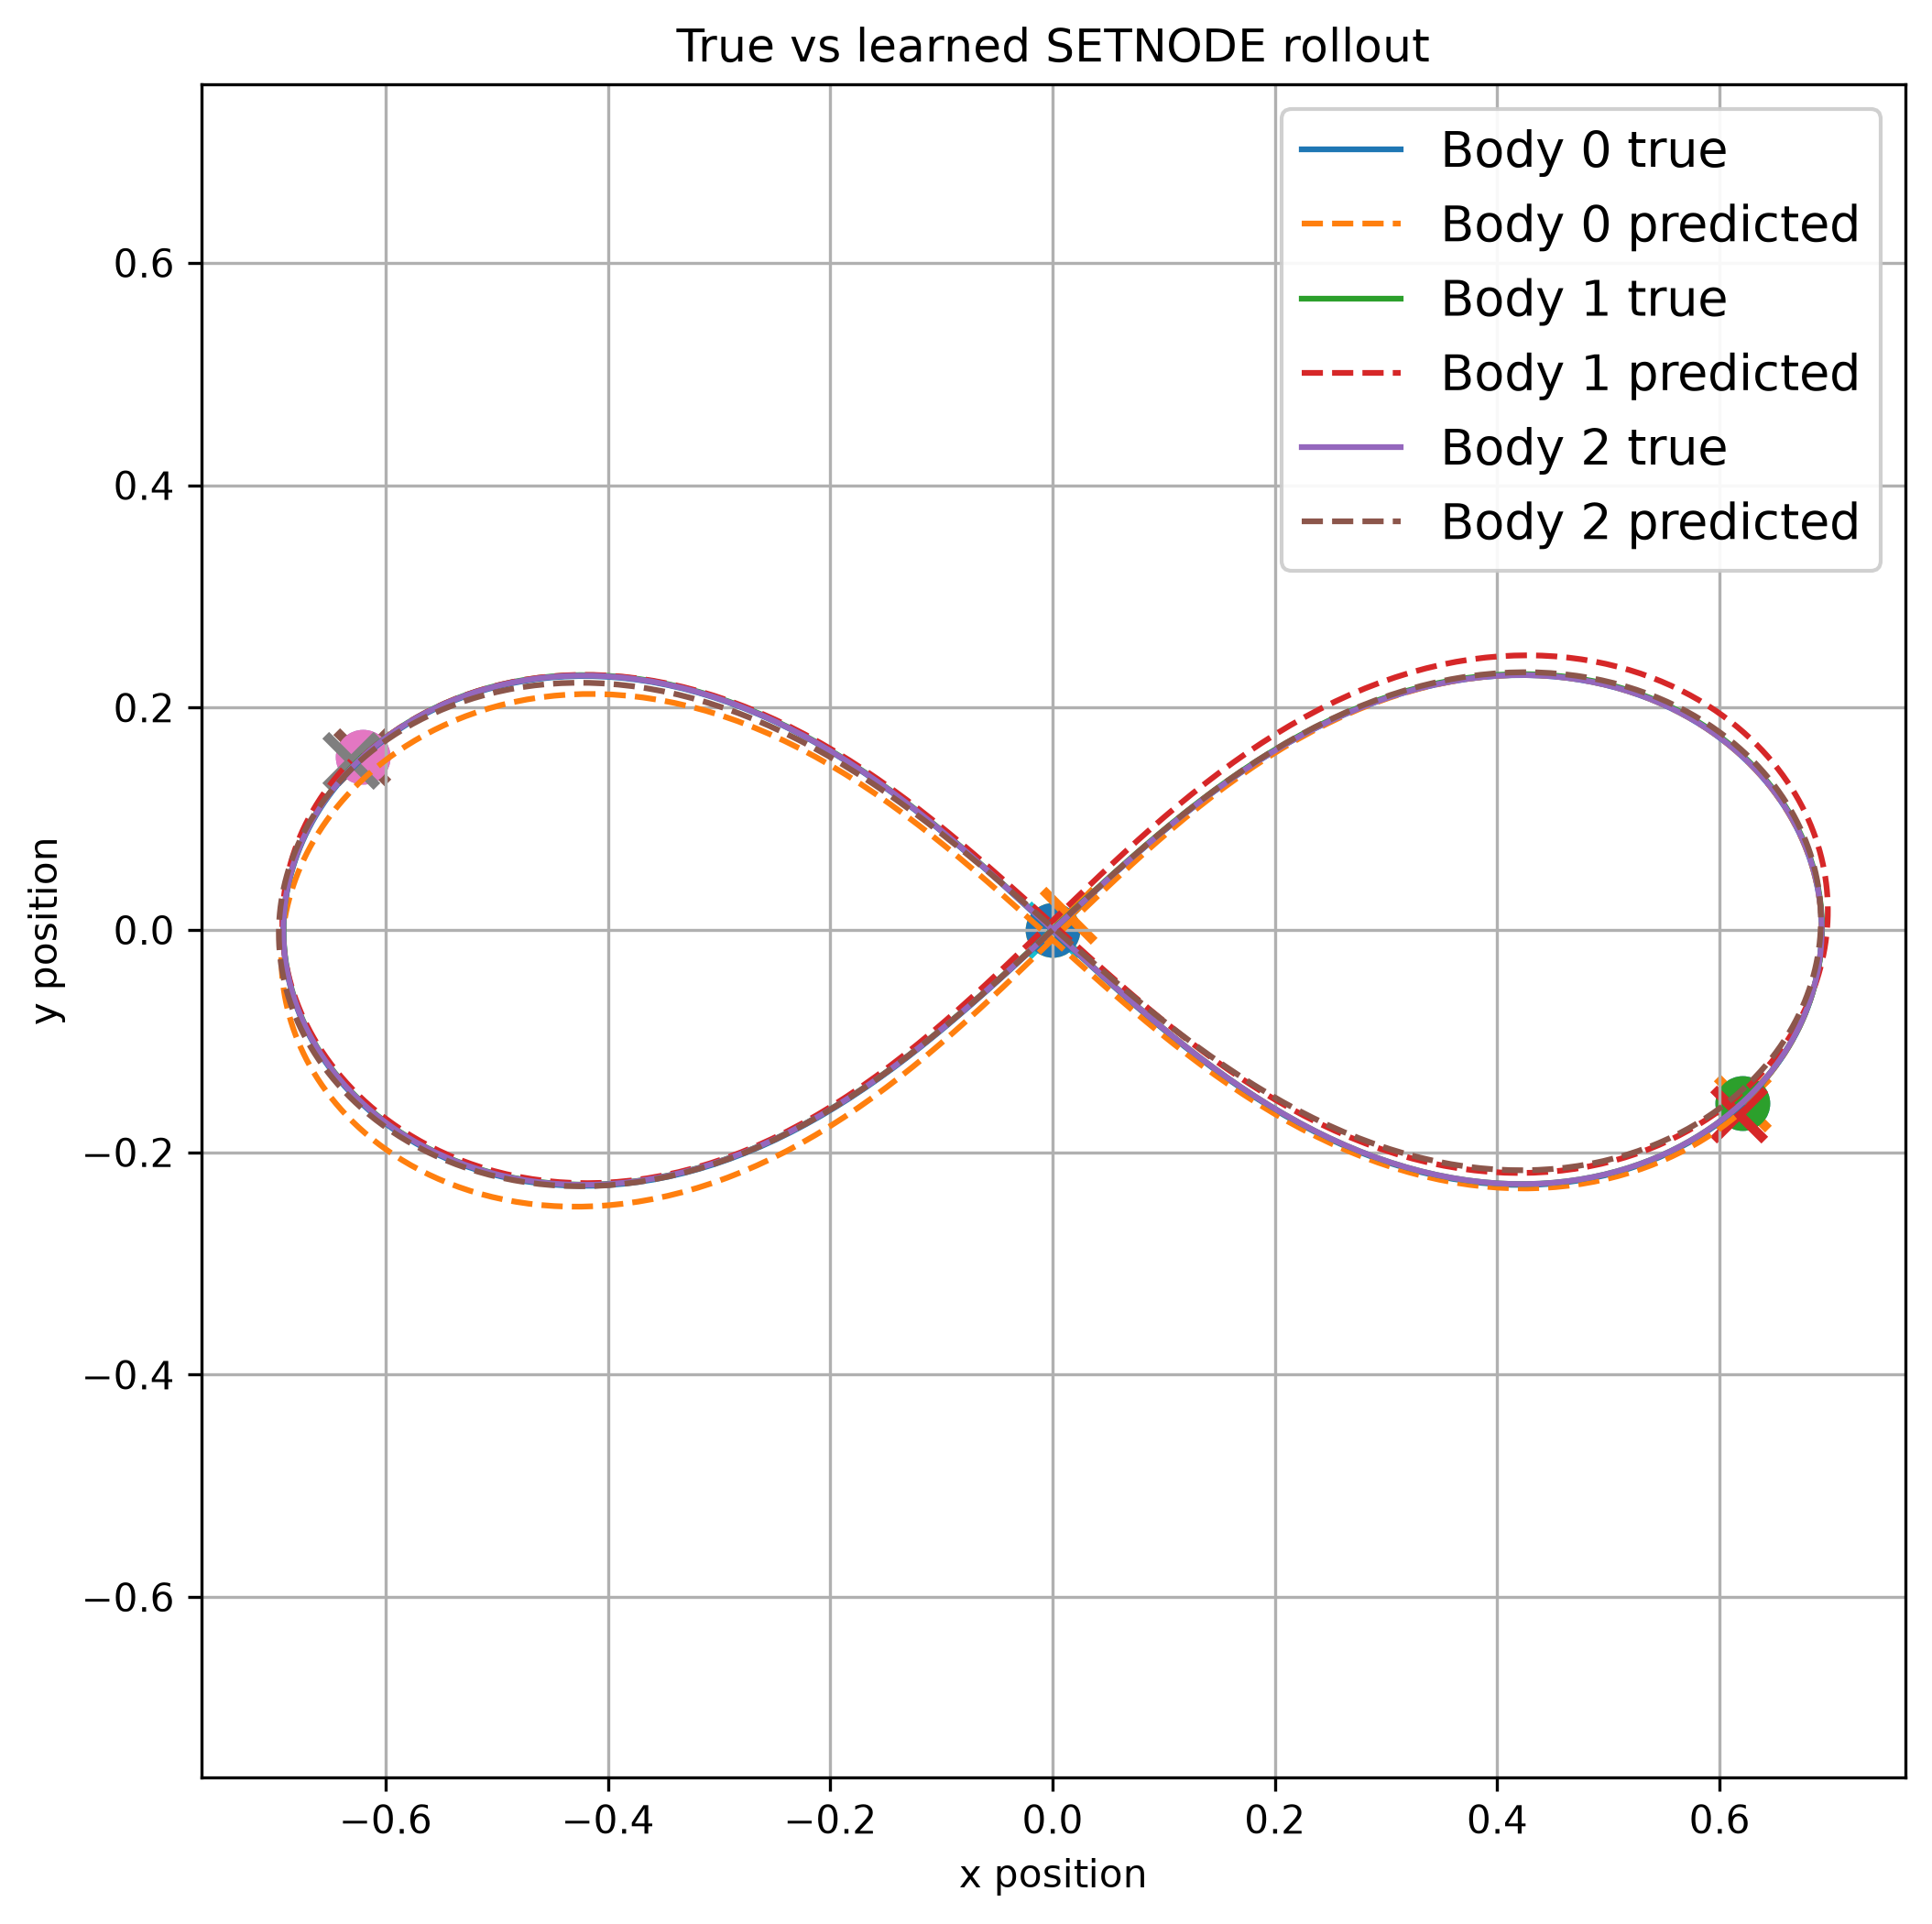
\includegraphics[width=\linewidth]{setnode_figure_eight.png}
        \caption{Figure-eight trajectory, $t=3.24$.}
        \label{fig:later_figure_eight}
    \end{subfigure}\hfill
    \begin{subfigure}[t]{0.49\textwidth}
        \centering
        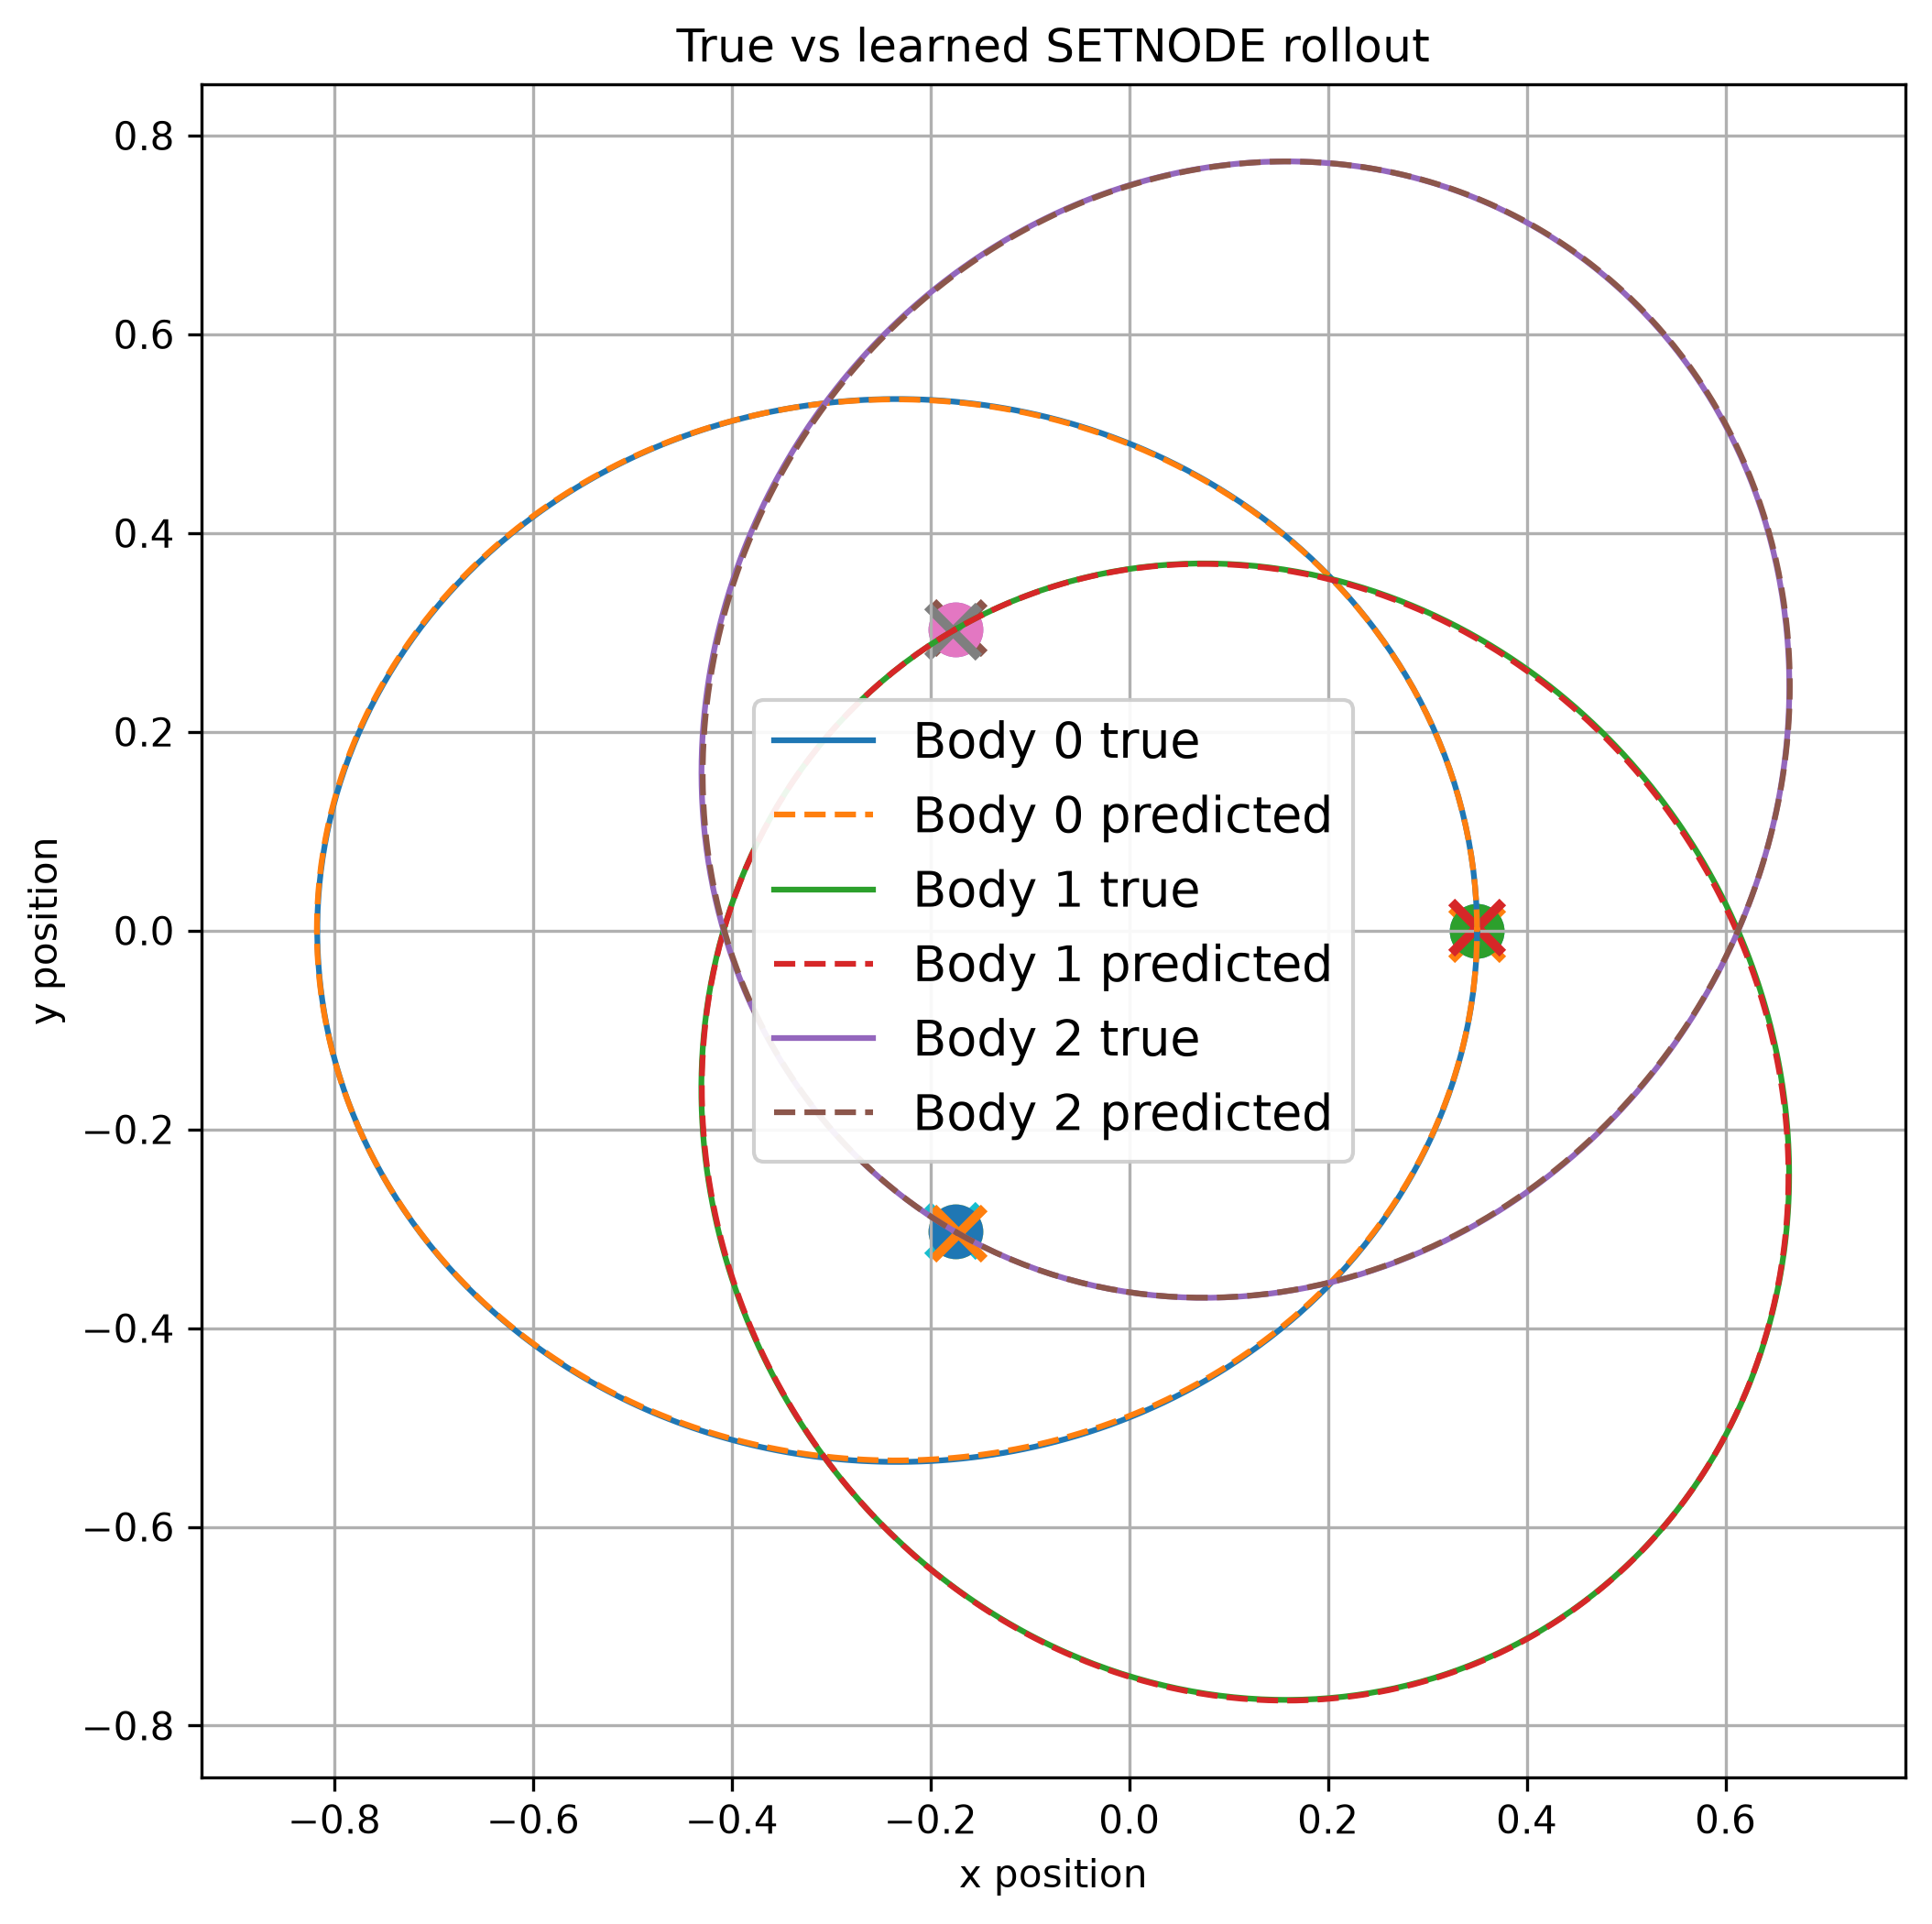
\includegraphics[width=\linewidth]{setnode_planar_orbit.png}
        \caption{Three-body orbital trajectory, $t=3.68$.}
        \label{fig:later_planar_orbit}
    \end{subfigure}
    \caption{\textbf{Illustrative rollouts with an extended SETNODE readout.}
    The models were trained for approximately 12 hours on a M3 Macbook Max and use scalar-score
    symmetrization, multiscale distance features, input-feature skip
    connections, and gated node, pair, and global contributions.
    Reference and predicted trajectories are overlaid; circles and crosses
    mark their respective positions at the displayed final time.
    These qualitative examples are separate from the four-hour quantitative
    evaluation.}
    \label{fig:later_rollouts}
\end{figure*}

\section{Discussion and Limitations}
\label{sec:discussion}

Our results support further study of the complete SETNODE design, but do not establish that
centered attention causes the improvement. EGNN-HNN has different depth, width, and other
implementation details; it is not SETNODE with attention removed. The models also differ in
supervised targets, inputs, and solvers. We cannot attribute the observed error differences to one
component alone.

The evidence covers one saved checkpoint per architecture and one fixed set of 50 test trajectories.
Trajectory-level standard deviations describe variation within that set. 
The suite uses only part of the 450-trajectory test partition. We have not established
a robust architecture ranking or generalization to different particle counts, mass distributions,
or much longer horizons. The rejection thresholds also limit coverage of close encounters.

Our additive/context-sensitive division remains a design hypothesis. Both branches operate on
latent features, and neither is forced to learn a particular class of physical interactions. With
exactly two neighbors per particle, the present task does not test variable-neighborhood behavior.

Our priority is an exact ablation using the same SETNODE implementation: additive-only processing,
additive processing with ordinary attention, and additive processing with centered attention.
Removing the additive branch would test its role separately. These experiments should keep the
force objective, solver, split, and validation procedure fixed, use several training seeds, and
report differences in active parameters and computational cost. A geometric-only GNS variant
would help distinguish feature engineering from message-passing design. None of these ablation
results is reported here.

Implementation checks should also measure rotation and permutation equivariance, summed internal
force, and agreement between automatic differentiation and finite differences of the potential.
Our propositions establish mathematical properties but do not replace numerical tests of the
software. Rollout-fine-tuning code and separate checkpoints exist, but matching evaluation results
are outside this report.

For the fluid--boundary motivation in Section~\ref{sec:intro}, future experiments should measure
errors separately near walls and in the fluid interior while varying the prevalence of boundary
interactions in training. Those studies require appropriate boundary features and nonconservative
modeling. Other extensions include mass-ratio shifts, particle-count transfer, and
three-dimensional trajectories.

\section{Conclusion}

We developed SETNODE to combine physics-motivated additive aggregation with context-sensitive
centered attention and an invariant-potential force model. Our original width-64, one-block,
two-head checkpoint achieves a mean rollout position MSE of $8.92\times10^{-5}$ on the fixed
50-trajectory suite, with center-of-mass drift close to the numerical reference. Energy drift and overlapping error distributions qualify this result. Controlled ablations, repeated training, and
broader rollout tests are needed to determine which components provide reliable benefits.

\section*{Acknowledgments}

This work was conducted through The University of Southern Mississippi REU Site in Deep Learning
for Dynamical Systems. I thank Dr. Qingguang Guan and Dr. Zhifu Xie for their mentorship and
feedback. This material is based upon
work supported by the National Science Foundation REU Site under Grant (FAIN) 2447675.


\FloatBarrier
\clearpage
\onecolumn
% Compact display spacing in the single-column reference/appendix material.
\setlength{\abovedisplayskip}{6pt plus 2pt minus 2pt}
\setlength{\belowdisplayskip}{6pt plus 2pt minus 2pt}
\setlength{\abovedisplayshortskip}{3pt plus 1pt}
\setlength{\belowdisplayshortskip}{4pt plus 1pt minus 1pt}

\begin{thebibliography}{12}
\bibitem[Ali et~al.(2023)]{ali2023centered}
Ameen Ali, Tomer Galanti, and Lior Wolf.
\newblock Centered self-attention layers.
\newblock \emph{arXiv:2306.01610}, 2023.
\newblock \url{https://arxiv.org/abs/2306.01610}.

\bibitem[Battaglia et~al.(2018)]{battaglia2018relational}
Peter W. Battaglia et~al.
\newblock Relational inductive biases, deep learning, and graph networks.
\newblock \emph{arXiv:1806.01261}, 2018.

\bibitem[Chen et~al.(2018)]{chen2018neural}
Ricky T. Q. Chen, Yulia Rubanova, Jesse Bettencourt, and David K. Duvenaud.
\newblock Neural ordinary differential equations.
\newblock In \emph{Advances in Neural Information Processing Systems}, volume 31, 2018.

\bibitem[Greydanus et~al.(2019)]{greydanus2019hamiltonian}
Samuel Greydanus, Misko Dzamba, and Jason Yosinski.
\newblock Hamiltonian neural networks.
\newblock In \emph{Advances in Neural Information Processing Systems}, volume 32, 2019.

\bibitem[Liu et~al.(2024)]{liu2024segno}
Yang Liu, Jiashun Cheng, Haihong Zhao, Tingyang Xu, Peilin Zhao, Fugee Tsung, Jia Li, and Yu Rong.
\newblock SEGNO: Generalizing equivariant graph neural networks with physical inductive biases.
\newblock In \emph{International Conference on Learning Representations}, 2024.
\newblock \url{https://arxiv.org/abs/2308.13212}.

\bibitem[Sanchez-Gonzalez et~al.(2020)]{sanchezgonzalez2020learning}
Alvaro Sanchez-Gonzalez, Jonathan Godwin, Tobias Pfaff, Rex Ying, Jure Leskovec, and Peter Battaglia.
\newblock Learning to simulate complex physics with graph networks.
\newblock In \emph{ICML}, volume 119 of \emph{Proceedings of Machine Learning Research}, pages 8459--8468, 2020.

\bibitem[Satorras et~al.(2021)]{satorras2021en}
V{\'\i}ctor Garcia Satorras, Emiel Hoogeboom, and Max Welling.
\newblock E(n) equivariant graph neural networks.
\newblock In \emph{ICML}, volume 139 of \emph{Proceedings of Machine Learning Research}, pages 9323--9332, 2021.

\bibitem[Th{\"o}lke and De Fabritiis(2022)]{tholke2022equivariant}
Philipp Th{\"o}lke and Gianni De Fabritiis.
\newblock Equivariant transformers for neural network based molecular potentials.
\newblock In \emph{International Conference on Learning Representations}, 2022.
\newblock \url{https://arxiv.org/abs/2202.02541}.

\bibitem[Touvron et~al.(2021)]{touvron2021going}
Hugo Touvron, Matthieu Cord, Alexandre Sablayrolles, Gabriel Synnaeve, and Herv{\'e} J{\'e}gou.
\newblock Going deeper with image transformers.
\newblock In \emph{Proceedings of the IEEE/CVF International Conference on Computer Vision}, pages 32--42, 2021.

\bibitem[Vaswani et~al.(2017)]{vaswani2017attention}
Ashish Vaswani et~al.
\newblock Attention is all you need.
\newblock In \emph{Advances in Neural Information Processing Systems}, volume 30, 2017.

\bibitem[Veli{\v{c}}kovi{\'c} et~al.(2018)]{velickovic2018graph}
Petar Veli{\v{c}}kovi{\'c}, Guillem Cucurull, Arantxa Casanova, Adriana Romero, Pietro Li{\`o}, and Yoshua Bengio.
\newblock Graph attention networks.
\newblock In \emph{International Conference on Learning Representations}, 2018.
\bibitem[Ye et~al.(2025)]{ye2025differential}
Tianzhu Ye, Li Dong, Yuqing Xia, Yutao Sun, Yi Zhu, Gao Huang, and Furu Wei.
\newblock Differential transformer.
\newblock In \emph{International Conference on Learning Representations}, 2025.
\newblock \url{https://arxiv.org/abs/2410.05258}.
\end{thebibliography}
\clearpage

% References and appendices use one column for longer derivations.
\appendix
\section{Proofs of the Structural Properties}
\label{app:proofs}

We prove the propositions from Section~\ref{sec:properties} in the same order. All sums over
neighbors are taken over $j\in\cN(i)$. The derivative arguments assume the potential is
differentiable at the configurations involved. For the continuous-time results, model parameters
and particle masses are fixed, and the trajectory remains where the required derivatives exist.

\subsection{Proof of Proposition~\ref{prop:centered}: centered attention}
\label{proof:centered}

\begin{proof}
The softmax weights add to one. The $n_i$ uniform weights each equal $1/n_i$, so they also add to
one. Subtracting the two sums gives
\[
\sum_j\left(\alpha_{ij}^a-\frac{1}{n_i}\right)
=\sum_j\alpha_{ij}^a-\frac{n_i}{n_i}=1-1=0.
\]
Expanding the centered head in Equation~\eqref{eq:center} gives
\[
C_i^a=\sum_j\alpha_{ij}^aV^a(\widetilde e_{ij})
-\frac{1}{n_i}\sum_jV^a(\widetilde e_{ij}).
\]
The first term is the learned attention-weighted average and the second is the uniform average.
Finally, if every neighbor has the same value vector $V^a(\widetilde e_{ij})=c$, then
\[
C_i^a=c\sum_j\left(\alpha_{ij}^a-\frac{1}{n_i}\right)=0.
\]
Thus the head contributes no correction when all neighbor values are identical.
\end{proof}

\subsection{Proof of Proposition~\ref{prop:potential}: invariant potential}
\label{proof:potential}

\begin{proof}
We first consider a coordinate change $q_i'=Qq_i+b$. Translating both particles by the same vector
cancels in their relative position. Since $Q^\top Q=I$,
\[
\norm{q_j'-q_i'}^2
=\norm{Q(q_j-q_i)}^2
=(q_j-q_i)^\top Q^\top Q(q_j-q_i)
=\norm{q_j-q_i}^2.
\]
Every radial quantity used by the network is therefore unchanged. This includes the inverse-distance
feature and its numerical floor. The masses and their saved normalization statistics are also
unchanged, so the encoded node and edge features are the same.

Now follow the features through the network. The shared edge MLP receives the same inputs and
returns the same edge updates. The incoming sums, attention scores, centered heads, and node
updates therefore remain unchanged as well. Repeating this argument for each processing layer
shows that all latent features are unchanged. The final node and pair sums in
Equation~\eqref{eq:potential} give the same scalar $V_\theta$. Multiplication by the fixed scalar
$\sigma_F$ also preserves this equality, so
\[
\Uhat_\theta(Qq+b,m)=\Uhat_\theta(q,m).
\]

Next, permute the particles and their masses consistently. A node or edge then receives a different
label but carries the same physical data. Because the encoders and update functions share their
parameters across particles and edges, the intermediate representations are permuted in the same
way. A sum does not depend on the order of its terms, and neighbor-wise softmax permutes its
weights when its inputs are permuted.

The final node sum includes the same terms in a different order. Each unordered-pair term is also
unchanged: averaging the two directed messages removes the orientation of that pair. Hence the
potential satisfies $\Uhat_\theta(Pq,Pm)=\Uhat_\theta(q,m)$.
\end{proof}

\subsection{Proof of Proposition~\ref{prop:force}: equivariant force}
\label{proof:force}

\begin{proof}
Let $q'=Qq+b$. Proposition~\ref{prop:potential} gives
$\Uhat_\theta(Qq+b,m)=\Uhat_\theta(q,m)$. Differentiating with respect to the original particle
position $q_i$, the chain rule gives
\[
Q^\top\nabla_{q_i'}\Uhat_\theta(q',m)=\nabla_{q_i}\Uhat_\theta(q,m).
\]
Multiply by $Q$ and use $QQ^\top=I$:
\[
\nabla_{q_i'}\Uhat_\theta(q',m)=Q\nabla_{q_i}\Uhat_\theta(q,m).
\]
The force is the negative gradient of the potential. Negating the last equality therefore yields
$\Fhat_i(Qq+b,m)=Q\Fhat_i(q,m)$.

For particle permutations, regard $P$ as permuting the particle blocks of the stacked coordinate
vector. Applying the chain rule to $\Uhat_\theta(Pq,Pm)=\Uhat_\theta(q,m)$, with masses held fixed
with respect to coordinate differentiation, gives
\[
P^\top\nabla_{q'}\Uhat_\theta(q',Pm)=\nabla_q\Uhat_\theta(q,m),\qquad q'=Pq.
\]
Since $PP^\top=I$, multiplying by $P$ and negating gives
$\Fhat_\theta(Pq,Pm)=P\Fhat_\theta(q,m)$. Relabeling the particles therefore relabels their forces.
\end{proof}

\subsection{Proof of Proposition~\ref{prop:momentum}: momentum and center of mass}
\label{proof:momentum}

\begin{proof}
Translate every particle by $sc$, where $c\in\R^d$ is arbitrary and $s$ is a scalar translation
parameter. Translation invariance means
\[
\Uhat_\theta(q_1+sc,\ldots,q_N+sc,m)=\Uhat_\theta(q,m).
\]
The right-hand side does not depend on $s$. Differentiating at $s=0$ gives
\[
0=c^\top\sum_i\nabla_{q_i}\Uhat_\theta(q,m).
\]
This holds for every vector $c$, which is possible only if the summed gradient is zero. Because
$\Fhat_i=-\nabla_{q_i}\Uhat_\theta$, we obtain $\sum_i\Fhat_i=0$.

Total momentum is $p=\sum_i m_iv_i$. Using the equations of motion and constant masses,
\[
\frac{dp}{dt}=\sum_i m_i\dot v_i=\sum_i\Fhat_i=0.
\]
Thus momentum stays constant. The center of mass satisfies
\[
\dot q_{\rm cm}=\frac{\sum_i m_iv_i}{\sum_i m_i}
=\frac{p}{\sum_i m_i},\qquad \ddot q_{\rm cm}=0.
\]
It moves at constant velocity and remains fixed only when that velocity is initially zero.
\end{proof}

\subsection{Proof of Proposition~\ref{prop:energy}: learned energy}
\label{proof:energy}

\begin{proof}
We differentiate the kinetic and learned potential terms separately:
\[
\frac{d\widehat H}{dt}
=\sum_i m_iv_i^\top\dot v_i
+\sum_i\bigl(\nabla_{q_i}\Uhat_\theta\bigr)^\top\dot q_i.
\]
Substitute $m_i\dot v_i=\Fhat_i$, $\dot q_i=v_i$, and
$\nabla_{q_i}\Uhat_\theta=-\Fhat_i$:
\[
\frac{d\widehat H}{dt}
=\sum_i v_i^\top\Fhat_i-\sum_i\Fhat_i^\top v_i=0.
\]
The two sums are equal because each dot product is a scalar. Any change in kinetic energy is
therefore canceled by the change in the learned potential energy.
\end{proof}

This is a statement about the learned continuous-time system. It neither identifies the learned
potential with the true gravitational potential nor establishes exact energy conservation after
finite-step numerical integration.

\clearpage
\section{Experimental Record and Reproducibility}
\label{app:record}

\subsection{Archived checkpoints and evaluation records}

We use the six files named \texttt{one\_step\_115k\_4h.pt} in the \texttt{gns}, \texttt{egns},
\texttt{egnn\_hnn}, \texttt{hnn}, \texttt{setnode}, and \texttt{mlp} checkpoint directories. We read
the architecture settings, tensor shapes, target scales, validation criteria, and embedded split
manifests from these checkpoints. They contain the same original three-body split and the same
ordered validation-state list. The files \texttt{<model>\_test\_suite.json} supply the numerical
results. Their model-relative checkpoint paths and trajectory IDs match the archived model names
and test manifest, and their summaries agree with recomputation from the individual entries.

\begin{table}[htbp]
\centering\small
\caption{Additional saved SETNODE settings and checkpoint identifiers. The source bundle contains
full configurations and hashes.}
\label{tab:archive}
\setlength{\tabcolsep}{7pt}
\begin{tabular}{lr@{\qquad}lr}
\toprule
SETNODE setting & Value & Model & Checkpoint SHA-256 prefix\\
\midrule
Node / edge input dimensions & 1 / 2 & GNS & \texttt{8c3785e9b1}\\
Hidden layers per configurable MLP & 1 & EGNN & \texttt{23236a497e}\\
Attention heads / width per head & 2 / 32 & EGNN-HNN & \texttt{44c23e8052}\\
Feed-forward width & 128 & HNN & \texttt{3d635ef670}\\
Readout distance embedding & 8 & MLP & \texttt{1192eb5d2f}\\
Validation samples / seed & 500 / 1234 & SETNODE & \texttt{b293fea95e}\\
\bottomrule
\end{tabular}
\end{table}

\subsection{Source version and remaining gaps}

Our method description follows the \href{https://github.com/Branshi/REU-PhysicalAI}{REU-PhysicalAI}
source snapshot \texttt{32c05fe6} and the supplied MLP files found in snapshot \texttt{67a9d90}. This is the inspected source version,
not a verified historical training commit. The original checkpoint's normalization and validation
fields, together with the matching trainer, support the force objective.

The archive does not store exact training times, completed-update counts, the original execution
environment and commands, mass-sampling parameters,
and simulation/storage precision.  The large saved epoch limits are configured limits, not completed
epoch counts. We also do not infer the missing dataset settings from later code defaults.

The numerical analyses in this paper use archived evaluation records; we did not retrain the
models or rerun the physical rollouts for this analysis.
\end{document}
